%% ------------------------------------------------------------------------- %%
\section{Diferença entre a abordagem tradicional e TDD}
\label{sec:diferencas-tdd-e-tradicional}

% TODO colocar mesmo essa secao aqui? melhor levar isso pra analise depois

Criar classes com baixo acoplamento e alta coesão não é tarefa fácil. Por esse
motivo, é comum que, após algum tempo, os designs percam qualidade e sua
manutenção se torne difícil e, por consequência, cara.
Para evitar esse problema, desenvolvedores constantemente validam a qualidade do
design através de diferentes práticas, como revisões de código, programação
pareada, métricas de código etc. Praticantes de TDD acreditam que escrever
testes de unidades é útil também para validar a qualidade do design.

Em abordagens tradicionais de desenvolvimento de software, em que o teste é feito
apenas depois da funcionalidade ter sido completamente implementada, o
desenvolvedor acaba por perder o feedback dos testes durante a criação inicial
do design. Ao contrário, o praticante de TDD, por escrever testes
frequentemente, recebe feedback durante todo o processo de escrita do código.

A Figura \ref{fig:tdd-feedback} ilustra dois programadores, usando
abordagens diferentes, escrevendo pequenos pedaços de código para uma
funcionalidade. Praticantes de TDD validam constantemente o design por meio de
testes, o que não ocorre com praticantes de abordagens tradicionais, em que
muitos pequenos pedaços de código são escritos antes dos testes.

\begin{figure}[H]
  \centering
  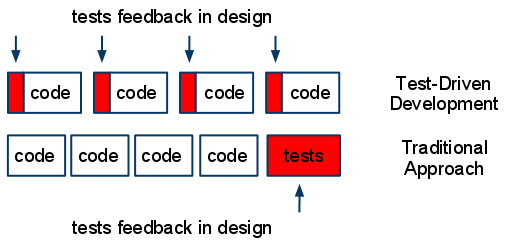
\includegraphics[scale=0.4]{tdd-and-traditional.png}
  \caption{Diferença do \textit{feedback} dos testes entre praticantes de TDD e
  praticantes de abordagens tradicionais}
  \label{fig:tdd-feedback}
\end{figure}

As informações dadas pelos testes sobre acoplamento e coesão são úteis para
guiar o design. Os testes provêm maneiras de comunicar o desenvolvedor sobre
possíveis problemas de design. 
